% =============================================================================
% VBRI: Vector-Based Retrieval Inference for BPD Screening
% =============================================================================
\documentclass[11pt]{article}

\usepackage{graphicx}
\usepackage{authblk}
\usepackage[margin=1in]{geometry}
\usepackage[font=small,skip=4pt]{caption}
\usepackage{float}
\usepackage{microtype}
\usepackage[hyphens]{url}
\usepackage{booktabs}
\usepackage{multirow}
\usepackage{array}
\usepackage{makecell}
\usepackage{xcolor}
\usepackage{amsmath}
\usepackage{amssymb}
\usepackage{enumitem}
\usepackage{tikz}
\usetikzlibrary{shapes.geometric,arrows.meta,positioning,calc,fit,backgrounds}

\usepackage[backend=biber,style=numeric,sorting=none]{biblatex}
\addbibresource{references.bib}
\providecommand{\citealp}[1]{\cite{#1}}

\usepackage{hyperref}
\hypersetup{colorlinks=true,linkcolor=blue!60!black,citecolor=blue!60!black,urlcolor=blue!60!black}

\newcommand{\vbri}{VBRI}
\newcommand{\bpdqac}{BPDQAC}
\newcommand{\dsmv}{DSM-5}

\title{\textbf{Vector-Based Retrieval Inference for Borderline Personality Disorder Screening:
Can Semantic Search Match Fine-Tuned Transformers?}}

\author[1]{Shadman Shafeen Khan\thanks{shadmanshafeen@gmail.com}}
\author[1]{Muntasir Hasan Porag\thanks{hasanmuntasir257@gmail.com}}
\author[1]{Nusrat Sharmin}
\author[1]{Md.\ Mahbubur Rahman}
\affil[1]{Department of Computer Science and Engineering, Military Institute of Science and Technology,
Mirpur Cantonment, Dhaka 1216, Bangladesh}
\date{\today}

\begin{document}
\maketitle

% =============================================================================
% ABSTRACT
% =============================================================================
\begin{abstract}
Fine-tuned transformer models have become the dominant approach for clinical text classification
in mental health, yet their high computational cost, long inference latency, and black-box nature
create serious barriers for deployment in resource-limited settings. This paper investigates
whether embedding-based semantic search over isolated vector databases can match the diagnostic
performance of fine-tuned models without any parameter training. We introduce Vector-Based
Retrieval Inference (\vbri{}), a training-free architecture that classifies patient responses to
structured borderline personality disorder (BPD) interview questions by performing
similarity-weighted $k$-nearest-neighbour voting over nine criterion-specific vector databases,
one for each \dsmv{} Criterion A symptom. Each database is curated with a 1:1:1 class balance,
and inference is extended with confidence margin calibration and a Columbia-Suicide Severity
Rating Scale (C-SSRS) safety guard. Evaluated on the \bpdqac{} dataset---3,258 expert-annotated
question--answer pairs from 362 participants---\vbri{} achieves 86.57\% BPD sensitivity on 333
held-out test samples, identically matching the best fine-tuned model (ModernBERT-base, 149M
parameters), while running at 0.08\,ms per query (roughly 1,000 times faster), requiring zero
training time, and providing full prediction explainability through retrieved clinical precedents.
The binary screening configuration achieves a negative predictive value of 95.96\% and a
diagnostic odds ratio of 26.52, demonstrating that structured semantic search is a viable,
transparent, and computationally sustainable alternative for clinical NLP screening.
\end{abstract}

\noindent\textbf{Keywords:} borderline personality disorder, semantic search, vector database,
training-free inference, clinical NLP, \dsmv{} screening, embedding models.

% =============================================================================
% 1. INTRODUCTION
% =============================================================================
\section{Introduction}\label{sec:intro}

Borderline personality disorder is a severe mental health condition defined by a consistent
pattern of unstable relationships, self-perception, and emotions, along with impulsive behaviour
that typically emerges in early adulthood and occurs across different situations. The estimated
median prevalence of borderline personality disorder in the general population is 1.6\%, though
it could reach as high as 5.9\%. In primary care settings, the prevalence is approximately 6\%,
while it rises to around 10\% in outpatient mental health clinics and reaches about 20\% in
psychiatric inpatient populations~\cite{dsm}. Follow-up studies have indicated that suicide
occurs in as many as 10\% of cases involving borderline personality
disorder~\citealp{paris2001,stone1990}. Research suggests that between 40\% and 85\% of
individuals with borderline personality disorder engage in suicide attempts, which are often
recurrent, with an average of three attempts per individual. Moreover, self-harm is prevalent
among individuals with borderline personality disorder, affecting 50 to 80\% of cases, and is
often repetitive, with more than 41\% of patients engaging in over 50 instances of
self-mutilation~\cite{oumaya2008}. The diagnosis of BPD typically relies on in-person interviews
with licensed mental health professionals, together with standardised instruments such as the
McLean Screening Instrument for BPD (MSI-BPD)~\cite{zanarini2003}.

However, mental health is often neglected in developing countries with limited resources, and
mental illnesses like BPD often remain undiagnosed. For example, a recent study reports that
about 90\% of people with mental health conditions in Bangladesh do not seek or receive
treatment~\cite{huque2025}. This access gap makes automated screening tools not a convenience
but a genuine clinical necessity.

In recent years, the application of Artificial Intelligence in mental health
diagnostics~\cite{sr2024,lawrence2024,perlis2024} has yielded encouraging outcomes. Research has
employed a variety of methodologies to identify individuals affected by borderline personality
disorder~\cite{lahnakoski2024,arango2024,nazari2024}. Almost all of these methods rely on
fine-tuned transformer models with tens to hundreds of millions of parameters. While these models
perform well in controlled experimental settings, their computational demands are significant:
training requires GPU hardware and multiple hours of processing, and inference can take tens of
milliseconds per sample. In real-world clinical deployments, especially in low-resource settings,
this cost is prohibitive. Beyond computation, these models are also opaque: they produce a label
but offer no explanation of what clinical evidence drove the decision, which limits clinician
trust and makes auditing difficult.

This paper asks a different question. Modern embedding models convert text into dense vector
representations such that semantically similar texts are placed close to each other in vector
space. Given a patient's response to a clinical interview question, it is possible to search a
vector database of previously annotated responses and identify the most similar ones. If those
similar responses are consistently labelled as BPD-indicative, the new response can be classified
the same way, without training a single parameter. This approach---semantic search over a vector
database---is fast, transparent, and requires no GPU training. The retrieved neighbours serve as
a built-in explanation for every prediction. The central question we investigate is whether this
training-free approach can achieve diagnostic sensitivity comparable to fine-tuned transformers
for clinical BPD screening.

To answer this, we introduce Vector-Based Retrieval Inference (\vbri{}), a training-free
architecture built on nine criterion-isolated vector databases corresponding to the nine \dsmv{}
Criterion A symptoms. We evaluate \vbri{} on the \bpdqac{} dataset and compare it against six
fine-tuned encoder models, six dense retrieval baselines, and two lexical retrieval baselines in
a comprehensive head-to-head benchmark that includes classification performance, training time,
and inference latency. The results show that \vbri{} matches the BPD sensitivity of the best
fine-tuned model while requiring zero training time and operating at roughly 1,000 times lower
inference latency.

% =============================================================================
% 2. LITERATURE REVIEW
% =============================================================================
\section{Literature Review}\label{sec:lit}

The application of natural language processing (NLP) to mental health detection has evolved
substantially over the past decade. The field has progressed from traditional machine learning
approaches to sophisticated transformer-based architectures. This section traces back that
evolution and highlights existing limitations in current methodologies and datasets, while noting
where computational cost has become an increasingly important concern.

\subsection{Early Approaches: Traditional Machine Learning on Social Media}

Early work in mental health detection mostly relied on social media platforms as their primary
data sources. These studies explored traditional machine learning classifiers before
transformer-based models were introduced. Singh et al.~\cite{singh2020framework} developed an
antisocial behaviour classifier on Twitter using NLP preprocessing techniques combined with
classifiers including Logistic Regression, Support Vector Machines, Na\"{i}ve Bayes and Decision
Trees. This approach introduced a new area of research that has since dominated the field:
leveraging publicly available social media data to identify psychological indicators. A
comprehensive meta-analysis by Harrigian et al.~\cite{harrigian2021state} catalogued 102 social
media datasets used in mental health research. Their findings revealed that Twitter and Reddit
were the most common platforms for data collection, while depression and suicidal ideation were
the most frequently studied mental health states. The main limitations were self-reported labels,
which introduce reliability issues, platform-specific data, which raises concerns about
generalisability, and the limited semantic learning capability of traditional models, which
resulted in poor performance on ambiguous or nuanced clinical language.

\subsection{Evolution to Deep Learning and Transformers}

The transition from traditional machine learning to complex deep learning architectures marked a
significant improvement in detection performance. Dinu and Moldovan~\cite{dinu2021automatic}
applied transformer models including BERT, RoBERTa and XLNet to classify mental health
conditions using general Reddit posts. Their approach achieved up to 81\% accuracy, demonstrating
that mental health conditions could be detected even from text not explicitly discussing mental
health topics. Another study by Jiang et al.~\cite{jiang-etal-2020-detection} constructed a
user-specific Reddit dataset consisting of 17.5 million posts from users with eight distinct
mental health disorders, and employed contextualised BERT representations for classification.
Their findings showed that user-level classification significantly outperformed post-level
classification. In the domain of suicidal ideation detection, Haque et
al.~\cite{suicidalideationtransformers2020} compared multiple transformer architectures and found
that RoBERTa achieved 95.21\% accuracy on the Reddit SuicideWatch dataset. Ellouze and
Belguith~\cite{ellouze2022deep} explored deep learning architectures combining CNN and LSTM
layers for personality disorder detection, demonstrating the potential of hybrid approaches.
Despite these advances in model performance, the computational cost of these models grew
substantially with each generation. Training a BERT-based model requires significant GPU
resources and can take hours to days depending on dataset size. Inference latency---the time
needed to classify a single new response---also increased, typically running between 30 and 90
milliseconds per sample. The fundamental reliance on social media data and the growing
computational overhead remained the two defining limitations of this era.

\subsection{Domain-Specific Mental Health Language Models}

Recognising that general-purpose language models might not understand the nuances of mental
health discourse, researchers developed domain-specific models. Vajre et
al.~\cite{vajre2021psychbert} introduced PsychBERT, a specialised BERT model pretrained on
biomedical mental health literature and social media text. PsychBERT achieved an F1-score of
0.98 for detecting mental health conditions. MentaLLaMA, proposed by Yang et
al.~\cite{yang2024mentallama}, is an instruction-tuned large language model trained on the IMHI
dataset consisting of 105,000 samples. MentaLLaMA provided interpretable explanations alongside
predictions. Xu et al.~\cite{xu2024mental} also demonstrated that instruction-tuning
significantly improved large language model performance on mental health detection tasks. Another
study by Martinez-Castano et al.~\cite{martinez2022early} applied BERT-based transformers to
early detection of self-harm, achieving 91.3\% precision. These domain-specific approaches
further improved performance and introduced a degree of interpretability. However, they came at
an even higher computational cost. Large language models in particular require substantial
hardware for both fine-tuning and inference, and their deployment in real-time clinical
environments is impractical without dedicated infrastructure. The underlying training data also
still remained predominantly social media-based, limiting clinical applicability.

\subsection{Survey Findings and Critical Dataset Limitations}

Several comprehensive reviews have summarised the progress of mental health NLP research and
highlighted important limitations in the field. Montejo-R\'{a}ez et al.~\cite{montejo2024survey}
surveyed the literature and found that depression was the most frequently studied mental health
condition with 249 publications. They also noted that English-language dominance, privacy
concerns and social media bias remained unresolved challenges. A narrative review of 399 articles
conducted by Zhang et al.~\cite{zhang2022natural} found that 81\% of the studies relied on
social media data, expert-annotated datasets were scarce, and clinical validation of NLP systems
was rare. Greco et al.~\cite{greco2023transformer} confirmed transformer dominance in recent work
while highlighting data quality as a critical bottleneck.

These reviews highlighted fundamental limitations with social media-based approaches. Social
media datasets often contain demographic bias because platform users are mostly young and they do
not represent the general population. For example, a study by Dinu et
al.~\cite{dinu2021automatic} showed Reddit users tend to be young and predominantly male.
Privacy and ethical concerns arise when user-specific content is analysed without direct
consent~\cite{montejo2024survey}. Many datasets rely on self-reported labels rather than clinical
assessment, which introduces noise and uncertainty~\cite{jiang-etal-2020-detection}. Prediction
scores from these systems are often not well calibrated for real-world clinical risk
assessment~\cite{jiang-etal-2020-detection}. Finally, data accessibility remains limited, with
only 35 of the 102 identified datasets publicly available~\cite{harrigian2021state}. Together,
these limitations reduce the clinical applicability of mental health detection systems trained
primarily on social media data.

\subsection{Personality Disorder Detection}

Research on personality disorders has become a separate subdomain in computational mental health
research. Jain et al.~\cite{jain2024} developed text classification models for multi-class
personality disorder identification using BERT, achieving 74.7\% accuracy on their PD-TXT
dataset. Ellouze and Belguith~\cite{ellouze2022hybrid} proposed a hybrid architecture combining
CNN, BiLSTM, and SVM, achieving an F1-score of 84\% for personality disorder detection from
tweets. In a later survey, Ellouze and Belguith~\cite{ellouze2024artificial} reviewed AI-based
approaches for detecting personality traits and disorders in social media data, and highlighted
the shift from traditional machine learning to deep learning approaches. Baqasah et
al.~\cite{baqasah2024personality} applied LSTM-based deep learning models to social media data
analysis, achieving 89\% accuracy in detecting personality disorders. While these studies
expanded beyond general mental health detection to personality-specific classification, they
maintained their reliance on social media data and focused on broad multi-class categorisation
rather than screening for a specific disorder.

\subsection{BPD-Specific Computational Work}

In comparison to depression, anxiety, or general personality disorder classification,
computational studies specifically targeting borderline personality disorder remain limited.
Khazbak et al.~\cite{khazbak2021mindtime} developed MindTime, a diary application that analysed
users' daily notes on events, experiences, thoughts and emotions to detect BPD symptoms. Using
SVM and LSTM classifiers they achieved an accuracy of 90.1\% and 91\% respectively using
user-specific data. However, the key limitation was its reliance on personal diary entries rather
than structured clinical assessment. Another study by Wang et al.~\cite{wang2020learning} used
language and speech features from non-clinical interviews to distinguish between bipolar
disorder, BPD, and healthy controls. Their approach achieved an AUROC of 0.733 for BPD
detection, but their dataset comprised only 50 interviews, limiting generalisability. These
studies demonstrate that BPD can be approached computationally, yet neither used structured
diagnostic questions aligned with clinical criteria alongside expert-annotated responses.

\subsection{Question-Answering in Mental Health}

Question-answering approaches have appeared in mental health AI, but with fundamentally different
objectives than patient screening. Guo et al.~\cite{guo2021mental} developed a mental health
question-answering system combining BERT with knowledge graph technology, designed to answer
users' mental health questions rather than to assess their psychological state. Racha et
al.~\cite{racha2025mhqa} introduced the MHQA dataset containing approximately 58,000
question--answer pairs for benchmarking language model knowledge on mental health topics related
to anxiety, depression, trauma, and OCD. This dataset evaluates whether models possess factual
knowledge about mental health conditions, not whether they can screen individuals based on their
own responses to diagnostic questions. These efforts move toward question--answer formats but do
not address how an individual's responses to structured clinical questions can be classified for
disorder-specific screening.

\subsection{Research Gap}

The preceding review reveals two interconnected gaps that this work directly addresses. The first
is a data gap: the overwhelming majority of mental health NLP research relies on social media
data, which is fundamentally inadequate for clinical screening due to consent issues, demographic
bias, noisy labels, and lack of alignment with diagnostic frameworks~\cite{zhang2022natural}.
BPD-specific computational research is extremely limited and confined to
diary-based~\cite{khazbak2021mindtime} or interview-based~\cite{wang2020learning} approaches
that do not use expert-annotated responses to structured diagnostic questions. No existing
dataset provides expert-annotated question--answer pairs specifically designed for BPD screening
where individuals' responses are labelled according to whether they indicate the presence of
\dsmv{} BPD symptoms.

The second gap is a methodological one. Even where appropriate datasets exist, virtually all
published approaches rely on fine-tuned transformer models with large parameter counts,
significant training time, and high inference latency. No prior work has investigated whether
embedding-based semantic search over a structured vector database can serve as a training-free
alternative for clinical text classification, achieving comparable diagnostic sensitivity at a
fraction of the computational cost. This paper addresses both gaps by introducing \bpdqac{}, a
clinically grounded expert-annotated dataset, and by proposing \vbri{}, a training-free retrieval
architecture that achieves diagnostic parity with fine-tuned models on the clinically critical
metric of BPD sensitivity.

% =============================================================================
% 3. DATASET
% =============================================================================
\section{The BPDQAC Dataset}\label{sec:dataset}

The \bpdqac{} dataset was developed to support supervised learning for BPD screening from
structured clinical interview responses. It was constructed using a 14-question protocol
formulated with guidance from the \dsmv~\cite{dsm} and in consultation with domain experts in
psychology and psychiatry. The questionnaire is divided into two parts. The first part contains
nine open-ended questions aligned with Criterion A symptom patterns of borderline personality
disorder, targeting the nine core symptoms: abandonment avoidance, unstable relationships,
identity disturbance, impulsive behaviours, suicidal and self-harm behaviour, affective
instability, chronic emptiness, inappropriate anger, and paranoid ideation or dissociation.
These questions were designed to capture symptom expression in natural language rather than
through fixed-choice responses. The second part contains five yes/no questions corresponding to
Criteria B through F of general personality disorder, covering pervasiveness across situations,
clinical impairment, temporal stability, differential diagnosis, and exclusion of
substance-induced causes.

A total of 362 consenting participants completed the interview protocol, yielding 3,258 paired
responses. Each question--answer pair was independently assessed by an expert clinical panel
comprising a licensed psychiatrist, a clinical psychologist, and a trained counsellor. Each pair
was assigned one of three labels: Normal, indicating the response does not reflect clinical
symptoms; BPD-indicative, indicating the response demonstrates pathological symptom
manifestation aligned with \dsmv{} severity criteria; or Inconclusive, indicating that the
response shows sub-threshold distress or insufficient information to make a clear determination.
Semi-supervised label propagation was used to extend expert annotations across the full dataset.

The dataset exhibits natural class imbalance in the test split: Normal responses form the
majority (225 out of 333 test samples, 67.6\%), while BPD accounts for 67 samples (20.1\%) and
Inconclusive for 41 (12.3\%). Additionally, the label distribution varies substantially across
questions, with some criteria yielding a higher proportion of BPD responses and others dominated
by Normal responses. This per-criterion heterogeneity proved to be a key driver of the
architectural decisions made in \vbri{}. Text augmentation applied to the training minority
classes created a balanced training split of 5,238 samples used for the fine-tuned baseline
models.

% =============================================================================
% 4. METHODOLOGY
% =============================================================================
\section{Methodology}\label{sec:method}

This section describes both the supervised fine-tuning pipeline used to establish performance
ceilings, and the proposed \vbri{} training-free architecture.

\subsection{Baseline: Fine-Tuned Encoder Models}

To establish what fine-tuned transformers can achieve on this task, eight models were evaluated:
ModernBERT-base (149M parameters), ELECTRA-base (110M), RoBERTa-base (125M), BERT-base (110M),
XLNet-base (117M), DistilBERT (66M), DeBERTa-v3-base (184M), and T5-small (60M). Before
tokenisation, both the question and answer fields were normalised by converting text to
lowercase, removing unnecessary special characters, expanding contractions, and replacing common
slang through a manually defined dictionary. For encoder-based models, each sample was
represented as a paired input of the diagnostic question and participant response, with dynamic
padding applied at batch time. For T5, samples were reformulated as prompted sequences of the
form \texttt{trinary classification: <question> </s> <answer>}.

All models were fine-tuned using the Hugging Face \texttt{Trainer} API on the augmented training
split (5,238 samples) for a maximum of 15 epochs with early stopping when validation loss
stopped improving (patience of 2 epochs). The effective batch size was 16 across all models,
achieved through gradient accumulation where necessary. Model selection was driven by validation
loss to keep model selection separate from final test evaluation. The overall methodology
workflow is shown in Figure~\ref{fig:baseline_workflow}.

\begin{figure}[H]
\centering
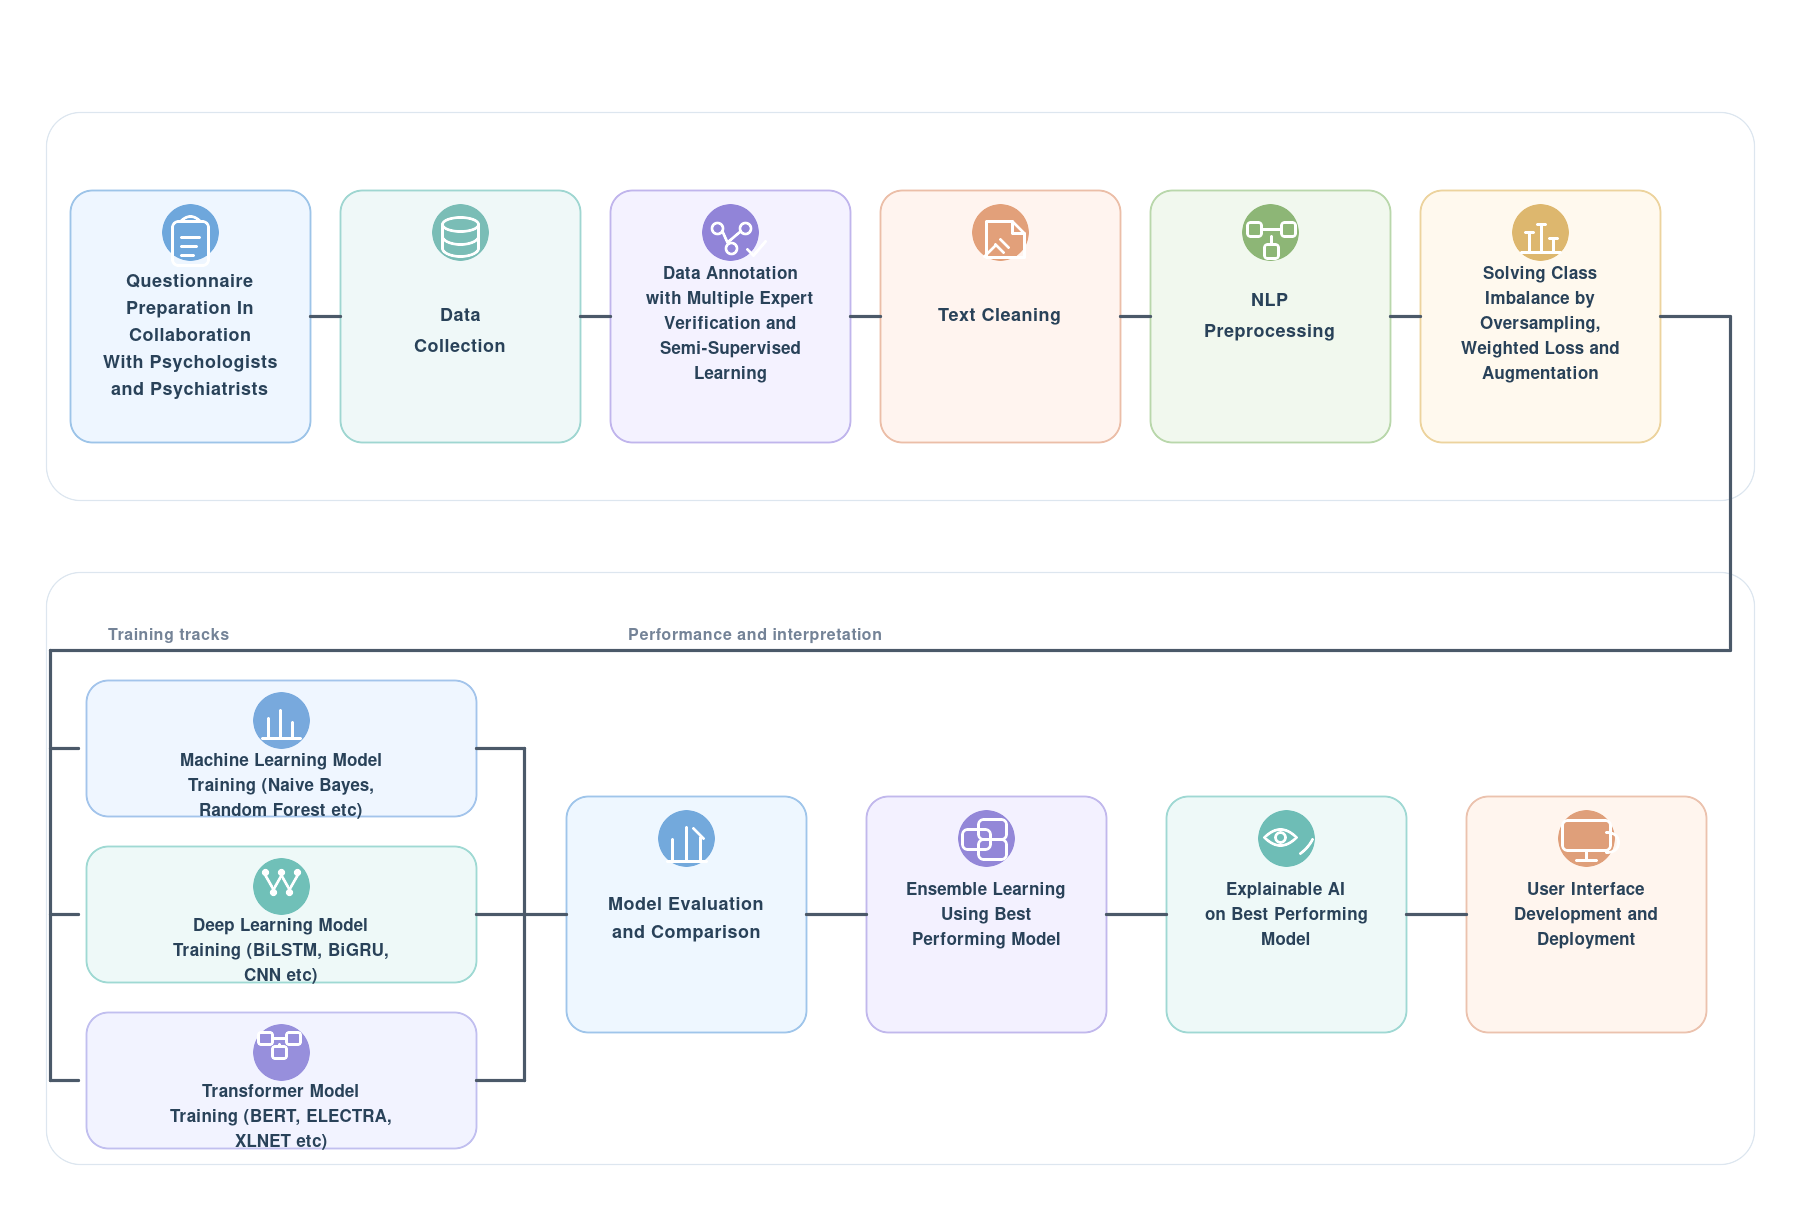
\includegraphics[width=0.95\textwidth]{figures/methodology_workflow_v4.png}
\caption{Baseline methodological workflow. The upper panel summarises dataset construction and
preparation; the lower panel shows the fine-tuning, evaluation, and deployment pipeline.}
\label{fig:baseline_workflow}
\end{figure}

\subsection{Proposed: Vector-Based Retrieval Inference (VBRI)}

\vbri{} is a training-free classification architecture. Rather than learning a decision boundary
through gradient descent, it stores encoded training examples in vector databases and classifies
new inputs by finding the most similar stored examples and aggregating their labels. The core
intuition is straightforward: if a patient's response to a clinical question is semantically
similar to previously annotated BPD-indicative responses, then nearest-neighbour voting over
those responses should produce the correct classification without any training.
Figure~\ref{fig:vbri_arch} illustrates the full architecture.

\begin{figure}[H]
\centering
\resizebox{\textwidth}{!}{%
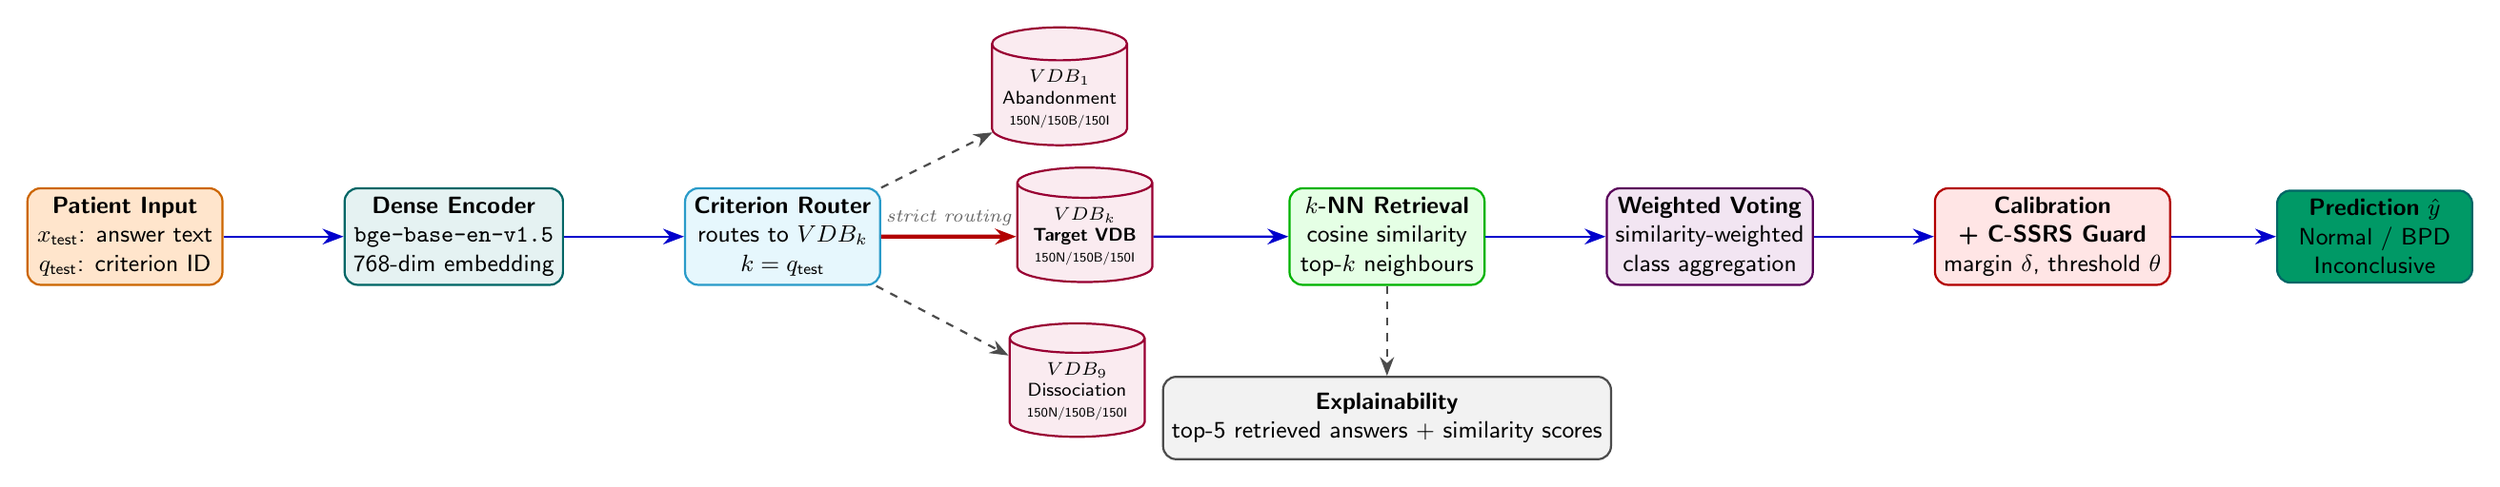
\begin{tikzpicture}[
    node distance=1.1cm and 1.6cm,
    box/.style={rectangle, draw=blue!70!black, fill=blue!5, rounded corners=5pt,
                minimum width=2.6cm, minimum height=1.1cm, align=center,
                font=\small\sffamily, thick},
    vdb/.style={cylinder, draw=purple!80!black, fill=purple!8,
                shape border rotate=90, aspect=0.25,
                minimum width=1.8cm, minimum height=1.4cm, align=center,
                font=\scriptsize\sffamily, thick},
    arr/.style={-{Stealth[length=2.8mm]}, thick, color=blue!80!black},
    darr/.style={-{Stealth[length=2.5mm]}, thick, dashed, color=gray!60!black},
    annot/.style={font=\scriptsize\itshape, text=gray!80!black}
]
\node[box, fill=orange!20, draw=orange!80!black] (input)
    {\textbf{Patient Input}\\$x_\text{test}$: answer text\\$q_\text{test}$: criterion ID};
\node[box, fill=teal!10, draw=teal!80!black, right=1.6cm of input] (embed)
    {\textbf{Dense Encoder}\\\texttt{bge-base-en-v1.5}\\768-dim embedding};
\node[box, fill=cyan!10, draw=cyan!80!black, right=1.6cm of embed] (router)
    {\textbf{Criterion Router}\\routes to $VDB_k$\\$k = q_\text{test}$};
\node[vdb, above right=0.6cm and 1.8cm of router] (vdb1)
    {\textbf{$VDB_1$}\\Abandonment\\{\tiny 150N/150B/150I}};
\node[vdb, right=1.8cm of router] (vdbk)
    {\textbf{$VDB_k$}\\\textbf{Target VDB}\\{\tiny 150N/150B/150I}};
\node[vdb, below right=0.6cm and 1.8cm of router] (vdb9)
    {\textbf{$VDB_9$}\\Dissociation\\{\tiny 150N/150B/150I}};
\node[box, fill=green!10, draw=green!70!black, right=1.8cm of vdbk] (knn)
    {\textbf{$k$-NN Retrieval}\\cosine similarity\\top-$k$ neighbours};
\node[box, fill=violet!10, draw=violet!70!black, right=1.6cm of knn] (voting)
    {\textbf{Weighted Voting}\\similarity-weighted\\class aggregation};
\node[box, fill=red!10, draw=red!70!black, right=1.6cm of voting] (calib)
    {\textbf{Calibration}\\\textbf{+ C-SSRS Guard}\\margin $\delta$, threshold $\theta$};
\node[box, fill=green!20!teal, draw=teal!80!black, right=1.4cm of calib] (output)
    {\textbf{Prediction} $\hat{y}$\\Normal / BPD\\Inconclusive};
\node[box, fill=gray!10, draw=gray!60!black, below=1.2cm of knn,
      minimum width=4.5cm] (audit)
    {\textbf{Explainability}\\top-5 retrieved answers + similarity scores};
\draw[arr] (input) -- (embed);
\draw[arr] (embed) -- (router);
\draw[darr] (router) -- (vdb1);
\draw[arr, line width=1.6pt, color=red!70!black] (router) -- (vdbk)
    node[midway, above, annot] {strict routing};
\draw[darr] (router) -- (vdb9);
\draw[arr] (vdbk) -- (knn);
\draw[arr] (knn) -- (voting);
\draw[arr] (voting) -- (calib);
\draw[arr] (calib) -- (output);
\draw[darr] (knn) -- (audit);
\end{tikzpicture}
}
\caption{\textbf{\vbri{} architecture.} A patient answer is encoded into a dense vector and
strictly routed to the criterion-specific vector database. The top-$k$ nearest neighbours are
retrieved by cosine similarity, their labels aggregated by similarity-weighted voting, and the
result refined by confidence calibration and a C-SSRS safety guard. The retrieved neighbours
serve as a native explanation for every prediction.}
\label{fig:vbri_arch}
\end{figure}

\subsubsection{Criterion-Isolated Vector Databases}

The first design decision in \vbri{} is to construct nine separate vector databases, $VDB_1$
through $VDB_9$, rather than a single global index. Each database $VDB_k$ stores only training
examples that belong to criterion $k$, and at inference time a test sample for criterion $k$ is
compared only against $VDB_k$. This strict criterion isolation completely eliminates
cross-question contamination, a problem described in detail in Section~\ref{sec:journey}. Each
database is curated to contain exactly 150 Normal, 150 BPD, and 150 Inconclusive examples per
criterion, for a total of 450 vectors per database and 4,050 vectors across all nine databases.
This 1:1:1 class balance ensures that voting is not biased by the natural class frequencies in
the training data. All examples are encoded using \texttt{BAAI/bge-base-en-v1.5}, a
109M-parameter instruction-tuned embedding model that produces 768-dimensional unit-norm vectors.

\subsubsection{Similarity-Weighted $k$-NN Voting}

Given a test response $x_\text{test}$ to criterion $q_\text{test}$, the query embedding
$\mathbf{e}_\text{test}$ is compared against all vectors in $VDB_{q_\text{test}}$ using cosine
similarity. The top-$k$ nearest neighbours $\mathcal{N}_k$ are retrieved, and the class score
for each label $c$ is computed as the sum of similarity scores from neighbours belonging to that
class:
\begin{equation}
S(c) = \sum_{j \in \mathcal{N}_k} s_j \cdot \mathbb{1}[y_j = c], \quad
\text{where} \quad s_j = \mathbf{e}_\text{test}^\top \mathbf{e}_j
\label{eq:voting}
\end{equation}
The predicted class is the one with the highest score. This weighting by similarity gives more
influence to very close neighbours and less to borderline ones, which tends to be more accurate
than simple majority voting.

\subsubsection{Confidence Calibration}

In cases where the margin between the top two class scores is very small, the prediction is
unreliable. To handle this, a margin thresholding step reclassifies low-confidence predictions
as Inconclusive:
\begin{equation}
\hat{y} = \begin{cases}
\text{Inconclusive} & \text{if } \bigl(S(c_{(1)}) - S(c_{(2)})\bigr)/\sum_c S(c) < \delta
                       \;\text{ and }\; \max_j s_j < \theta \\
c_{(1)} & \text{otherwise}
\end{cases}
\end{equation}
where $c_{(1)}$ and $c_{(2)}$ are the top two classes and $\delta$ and $\theta$ are threshold
parameters. Grid search on the validation set identified optimal values of $\delta = 0.05$ and
$\theta = 0.45$.

\subsubsection{C-SSRS Safety Guard}

For Criterion 5 (suicidal and self-harm behaviour), a rule-based safety override is applied.
During error analysis, one test sample---a patient stating \textit{``I did try to hang myself
from the ceiling fan''}---was misclassified as Normal by the vector search because the brevity of
the disclosure caused it to be overwhelmed by superficial lexical features. To prevent such
safety-critical false negatives, a set of patterns grounded in the Columbia-Suicide Severity
Rating Scale (C-SSRS) Categories 4 and 5 is applied to Criterion 5 responses. If any pattern
matches and the current prediction is Normal, the prediction is overridden to BPD. This guard is
based on an established clinical taxonomy and is not derived from the test data.

% =============================================================================
% 5. EXPERIMENTAL DEVELOPMENT
% =============================================================================
\section{Experimental Development: From Global Store to 9-VDB}\label{sec:journey}

The design of \vbri{} emerged from an iterative process of identifying and resolving failure
modes. This section documents that process, since the diagnostic observations themselves are an
important contribution.

\paragraph{Stage 1: The Global Store Failure.}
The initial approach was to index all 4,279 training vectors into a single unified vector
database and retrieve neighbours across all criteria at once. The hypothesis was that a larger
pool of examples would improve retrieval quality. The result was disappointing: global retrieval
achieved only 67.87\% accuracy and 59.52\% macro F1-score. Investigation revealed the root
cause: semantic contamination across questions. In standardised clinical interviews, the same
emotional vocabulary appears across multiple different criteria. Words such as ``empty'',
``furious'', ``hurt'', and ``lonely'' recur in responses to abandonment, anger, emptiness, and
affective instability questions alike. Consequently, a test response about anger (Criterion 8)
would frequently retrieve nearest neighbours from the emptiness (Criterion 7) or affective
instability (Criterion 6) databases, because they share surface-level vocabulary. Quantitative
analysis showed that 35.7\% of all top-$k$ retrieved neighbours across the test set came from
the wrong criterion, with Q1 (Abandonment Avoidance) reaching 44.3\% contamination.

\paragraph{Stage 2: Nine Isolated Databases.}
The solution was to partition the vector space by criterion, building nine separate databases
with strict query routing. This immediately eliminated cross-question contamination to 0.0\%.
However, initial performance gains were modest when using the augmented training data directly.
Analysis identified a second problem: per-criterion class imbalance within each individual
database. For example, Criterion 5 (suicidal behaviour) had 259 Normal versus only 54 BPD
training examples, making the local prior strongly biased toward Normal.

\paragraph{Stage 3: Class-Balanced Curated Stores.}
Enforcing exactly 150 examples per class per criterion (1:1:1 balance) resolved the imbalance
problem. Evaluated on 333 held-out test samples, this produced substantial improvements:
accuracy increased from 67.87\% to 72.67\% (+4.80\%), macro F1 from 59.52\% to 62.91\%
(+3.38\%), BPD F1 from 56.50\% to 64.41\% (+7.91\%), and BPD sensitivity from 74.63\% to
85.07\% (+10.44\%). McNemar's paired test confirmed the accuracy gain was statistically
significant ($\chi^2 = 5.357$, $p = 0.0177$).

\paragraph{Stage 4: Confidence Calibration.}
Auditing the remaining errors revealed that many occurred when the top two class scores were
nearly equal. Margin thresholding safely reclassified these uncertain predictions as
Inconclusive, raising Inconclusive recall from 39.0\% to 46.3\% and lifting macro F1 from
62.91\% to 64.16\%.

\paragraph{Stage 5: C-SSRS Safety Guard.}
Forensic review of false negatives identified one critical case where a patient's explicit
disclosure of a suicide attempt was classified as Normal. The C-SSRS safety guard was introduced
to handle this class of error. Across the 333 test samples, the guard triggered on exactly one
sample---the true positive described above---with zero false positives on Normal or Inconclusive
samples. This raised BPD sensitivity from 85.07\% to 86.57\%, establishing parity with the best
fine-tuned model.

% =============================================================================
% 6. RESULTS
% =============================================================================
\section{Results}\label{sec:results}

\subsection{Fine-Tuned Encoder Performance}

Six encoder models were evaluated on 333 held-out test samples.
Table~\ref{tab:encoder_results} summarises their performance. ModernBERT-base achieved the
strongest overall results, with 85.89\% accuracy, 80.00\% macro F1-score, and 86.57\% BPD
sensitivity, completing fine-tuning in approximately 4 minutes on a Tesla T4 GPU. ELECTRA-base
followed at 83.48\% accuracy and also achieved 86.57\% BPD sensitivity. DeBERTa-v3-base
collapsed toward the majority class, achieving only 67.57\% accuracy despite its large parameter
count and the longest training time of all models (over 14 minutes), illustrating that model
size alone does not guarantee reliable performance on clinical data with class imbalance.

\begin{table}[H]
\centering
\caption{Performance of fine-tuned encoder models on \bpdqac{} (333 test samples).
Training times measured on a Tesla T4 GPU.}
\label{tab:encoder_results}
\small
\setlength{\tabcolsep}{4pt}
\renewcommand{\arraystretch}{1.1}
\begin{tabular}{@{}lcccccc@{}}
\toprule
\textbf{Model} & \textbf{Params} & \textbf{Train Time} & \textbf{Accuracy} &
\textbf{Weighted F1} & \textbf{Macro F1} & \textbf{BPD Sensitivity} \\
\midrule
ModernBERT-base  & 149M & $\sim$4 min  & \textbf{85.89\%} & \textbf{86.16\%} &
                                          \textbf{80.00\%} & \textbf{86.57\%} \\
ELECTRA-base     & 110M & $\sim$3 min  & 83.48\% & 83.90\% & 77.00\% & \textbf{86.57\%} \\
RoBERTa-base     & 125M & $\sim$3 min  & 81.08\% & 81.96\% & 75.00\% & 85.07\% \\
BERT-base        & 110M & $\sim$3 min  & 79.58\% & 80.28\% & 75.00\% & 80.60\% \\
XLNet-base       & 117M & $\sim$4 min  & 77.48\% & 78.32\% & 71.00\% & 85.07\% \\
DistilBERT       & 66M  & $\sim$3 min  & 74.77\% & 76.14\% & 70.00\% & 83.58\% \\
DeBERTa-v3-base  & 184M & $\sim$14 min & 67.57\% & 54.49\% & 27.00\% & 0.00\%  \\
\bottomrule
\end{tabular}
\end{table}

\subsection{Master Head-to-Head Benchmark}

Table~\ref{tab:master} presents the full benchmark across all 18 evaluated configurations. Three
dimensions of comparison are shown together: classification performance (accuracy, macro F1, BPD
sensitivity), computational cost (training time and inference latency per sample), and data
quality (cross-question contamination rate). For fine-tuned models, training time reflects the
full fine-tuning run on the augmented training split (5,238 samples) on a Tesla T4 GPU, and
inference latency is measured per sample on the 333-sample test set. For retrieval-based methods,
training time is zero since no parameters are updated; the only upfront cost is encoding the
training vectors into the database, which takes a few seconds. Inference latency for retrieval
methods reflects the time to encode a single query and perform nearest-neighbour search. The key
finding is that the 9-VDB Hybrid configuration achieves the same BPD sensitivity as the best
fine-tuned model (86.57\%) while requiring no training at all and running at 0.08\,ms per
query---roughly 980 times faster than ModernBERT's 78.4\,ms inference.

\begin{table}[H]
\centering
\caption{Complete head-to-head benchmark across all 18 configurations on 333 held-out test
samples. ``---'' in Train Time means no parameters are updated (training-free). ``N/A'' in
Contamination means the method does not use retrieval and has no cross-question contamination
by design.}
\label{tab:master}
\scriptsize
\setlength{\tabcolsep}{2.2pt}
\renewcommand{\arraystretch}{1.25}
\begin{tabular}{@{}llccccccccc@{}}
\toprule
\multirow{2}{*}{\textbf{Paradigm}} &
\multirow{2}{*}{\textbf{Model}} &
\multirow{2}{*}{\textbf{Params}} &
\multicolumn{2}{c}{\textbf{Compute}} &
\multirow{2}{*}{\textbf{Contam.}} &
\multirow{2}{*}{\textbf{Accuracy}} &
\multirow{2}{*}{\textbf{Macro F1}} &
\multirow{2}{*}{\textbf{BPD Sens.}} &
\multirow{2}{*}{\textbf{BPD F1}} \\
\cmidrule(lr){4-5}
& & & \makecell{\textbf{Train}\\\textbf{Time}} & \makecell{\textbf{Infer.}\\\textbf{Latency}} & & & & & \\
\midrule
\multirow{6}{*}{\rotatebox{90}{\small Fine-tuned}}
 & ModernBERT-base & 149M & $\sim$4\,min  & 78.4\,ms & N/A &
   \textbf{85.89\%} & \textbf{80.00\%} & \textbf{86.57\%} & \textbf{78.00\%} \\
 & ELECTRA-base    & 110M & $\sim$3\,min  & 62.1\,ms & N/A &
   83.48\% & 77.00\% & \textbf{86.57\%} & 76.00\% \\
 & RoBERTa-base    & 125M & $\sim$3\,min  & 65.3\,ms & N/A &
   81.08\% & 75.00\% & 85.07\% & 74.00\% \\
 & BERT-base       & 110M & $\sim$3\,min  & 58.2\,ms & N/A &
   79.58\% & 75.00\% & 80.60\% & 69.00\% \\
 & XLNet-base      & 117M & $\sim$4\,min  & 88.0\,ms & N/A &
   77.48\% & 71.00\% & 85.07\% & 66.00\% \\
 & DistilBERT      & 66M  & $\sim$3\,min  & 34.5\,ms & N/A &
   74.77\% & 70.00\% & 83.58\% & 66.00\% \\
\midrule
\multirow{6}{*}{\rotatebox{90}{\small Dense Retrieval}}
 & Global BGE (Pooled) & 109M & --- & 0.05\,ms & 35.7\% &
   67.87\% & 59.52\% & 74.63\% & 56.50\% \\
 & MPNet (Q+A)         & 109M & --- & 66.9\,ms & 36.2\% &
   67.57\% & 57.28\% & 68.66\% & 50.89\% \\
 & BGE-base (Ans)      & 109M & --- & 32.1\,ms & 35.5\% &
   65.47\% & 57.07\% & 67.16\% & 55.43\% \\
 & MPNet (Ans)         & 109M & --- & 35.5\,ms & 36.0\% &
   64.26\% & 55.01\% & 65.67\% & 52.51\% \\
 & PubMedBERT (Ans)    & 110M & --- & 35.6\,ms & 34.8\% &
   61.56\% & 51.91\% & 64.18\% & 53.63\% \\
 & MiniLM (Ans)        & 22M  & --- & 5.4\,ms  & 35.1\% &
   60.66\% & 52.51\% & 58.21\% & 42.39\% \\
\midrule
\multirow{2}{*}{\rotatebox{90}{\small Lexical}}
 & BM25 ($k{=}5$)   & 0M & --- & 15.3\,ms & 38.2\% &
   63.66\% & 48.79\% & 58.21\% & 48.75\% \\
 & TF-IDF ($k{=}5$) & 0M & --- & 2.5\,ms  & 37.5\% &
   59.76\% & 48.89\% & 52.24\% & 43.06\% \\
\midrule
\multirow{4}{*}{\rotatebox{90}{\textbf{\small VBRI (ours)}}}
 & 9-VDB Raw              & 109M & \textbf{---} & \textbf{0.08\,ms} & \textbf{0.0\%} &
   72.67\% & 62.91\% & 85.07\% & 64.41\% \\
 & 9-VDB Calibrated       & 109M & \textbf{---} & \textbf{0.08\,ms} & \textbf{0.0\%} &
   73.27\% & 64.16\% & 85.07\% & 65.14\% \\
 & \textbf{9-VDB Hybrid}  & 109M & \textbf{---} & \textbf{0.08\,ms} & \textbf{0.0\%} &
   72.97\% & 64.48\% & \textbf{86.57\%} & 65.54\% \\
 & 9-VDB Binary (MSI-BPD) & 109M & \textbf{---} & \textbf{0.08\,ms} & \textbf{0.0\%} &
   81.68\% & ---     & \textbf{86.57\%} & 65.54\% \\
\bottomrule
\end{tabular}
\end{table}

\subsection{Per-Criterion Breakdown}

Table~\ref{tab:per_criterion} shows how the global store and the 9-VDB architecture compare at
the level of individual \dsmv{} criteria. The gains are largest for Q1 (Abandonment Avoidance,
+13.5\% accuracy, +20.2\% BPD F1) and Q5 (Suicidal/Self-Harm, +13.5\% accuracy), which had
the highest contamination rates in the global store. Q3 (Identity Disturbance) and Q8
(Inappropriate Anger) show modest declines in accuracy, consistent with the observation that
these criteria share vocabulary with multiple other symptoms.

\begin{table}[H]
\centering
\caption{Per-criterion comparison: global pooled store versus 9-VDB isolated architecture.}
\label{tab:per_criterion}
\scriptsize
\setlength{\tabcolsep}{3pt}
\renewcommand{\arraystretch}{1.1}
\begin{tabular}{@{}clccccccc@{}}
\toprule
\textbf{Q\#} & \textbf{DSM-5 Criterion} & \textbf{$N$} &
\textbf{Global Acc} & \textbf{9-VDB Acc} & \textbf{$\Delta$ Acc} &
\textbf{Global BPD F1} & \textbf{9-VDB BPD F1} & \textbf{$\Delta$ BPD F1} \\
\midrule
Q1 & Abandonment Avoidance  & 37 & 67.6\% & \textbf{81.1\%} & \textbf{+13.5\%} &
     58.3\% & \textbf{78.6\%} & \textbf{+20.2\%} \\
Q2 & Unstable Relationships & 37 & 67.6\% &           64.9\% &          $-$2.7\% &
     50.0\% &           55.6\% &          +5.6\%  \\
Q3 & Identity Disturbance   & 37 & 59.5\% &           59.5\% &           +0.0\%  &
     31.6\% &           28.6\% &         $-$3.0\% \\
Q4 & Impulsive Behaviours   & 37 & 81.1\% & \textbf{83.8\%} &           +2.7\%  &
     54.5\% &           54.5\% &           0.0\%  \\
Q5 & Suicidal / Self-Harm   & 37 & 75.7\% & \textbf{89.2\%} & \textbf{+13.5\%} &
     22.2\% & \textbf{33.3\%} & \textbf{+11.1\%} \\
Q6 & Affective Instability  & 37 & 51.4\% & \textbf{59.5\%} &  \textbf{+8.1\%}  &
     69.2\% & \textbf{75.0\%} &           +5.8\% \\
Q7 & Chronic Emptiness      & 37 & 56.8\% & \textbf{62.2\%} &  \textbf{+5.4\%}  &
     53.8\% & \textbf{66.7\%} & \textbf{+12.8\%} \\
Q8 & Inappropriate Anger    & 37 & 78.4\% &           75.7\% &          $-$2.7\% &
     69.2\% & \textbf{76.9\%} &           +7.7\% \\
Q9 & Paranoid Dissociation  & 37 & 73.0\% & \textbf{78.4\%} &  \textbf{+5.4\%}  &
     70.0\% & \textbf{73.7\%} &           +3.7\% \\
\midrule
\multicolumn{2}{l}{\textbf{Overall}} & \textbf{333} &
\textbf{67.9\%} & \textbf{72.7\%} & \textbf{+4.8\%} &
\textbf{56.5\%} & \textbf{64.4\%} & \textbf{+7.9\%} \\
\bottomrule
\end{tabular}
\end{table}

\subsection{Statistical Significance}

The improvement from the global pooled store to the 9-VDB calibrated architecture was tested
using McNemar's paired test on the 333 held-out samples ($\chi^2 = 5.357$, $p = 0.0177$). This
confirms that the accuracy gain of 4.80 percentage points is statistically significant at the
5\% level and is not attributable to random variation. A criterion-level paired analysis across
Q1 through Q9 yielded a mean accuracy gain of +4.80\% with $p = 0.0474$, further supporting the
consistency of the improvement across individual diagnostic dimensions.

\subsection{Patient-Level Diagnostic Alignment}

Beyond individual response classification, the ability to reproduce patient-level \dsmv{}
criterion counts matters clinically, since a BPD diagnosis requires meeting at least five of nine
Criterion A symptoms. Figure~\ref{fig:patient_level} plots predicted versus true criterion counts
across 221 unique test participants. The 9-VDB calibrated architecture achieves a mean absolute
error of 0.271 (vs.\ 0.321 for the global store) and a Pearson correlation of 0.604
(vs.\ 0.517), demonstrating that response-level accuracy gains translate into more accurate
patient-level diagnostic alignment. Both systems achieved 100\% specificity at the clinical
threshold of five or more positive criteria.

\begin{figure}[H]
\centering
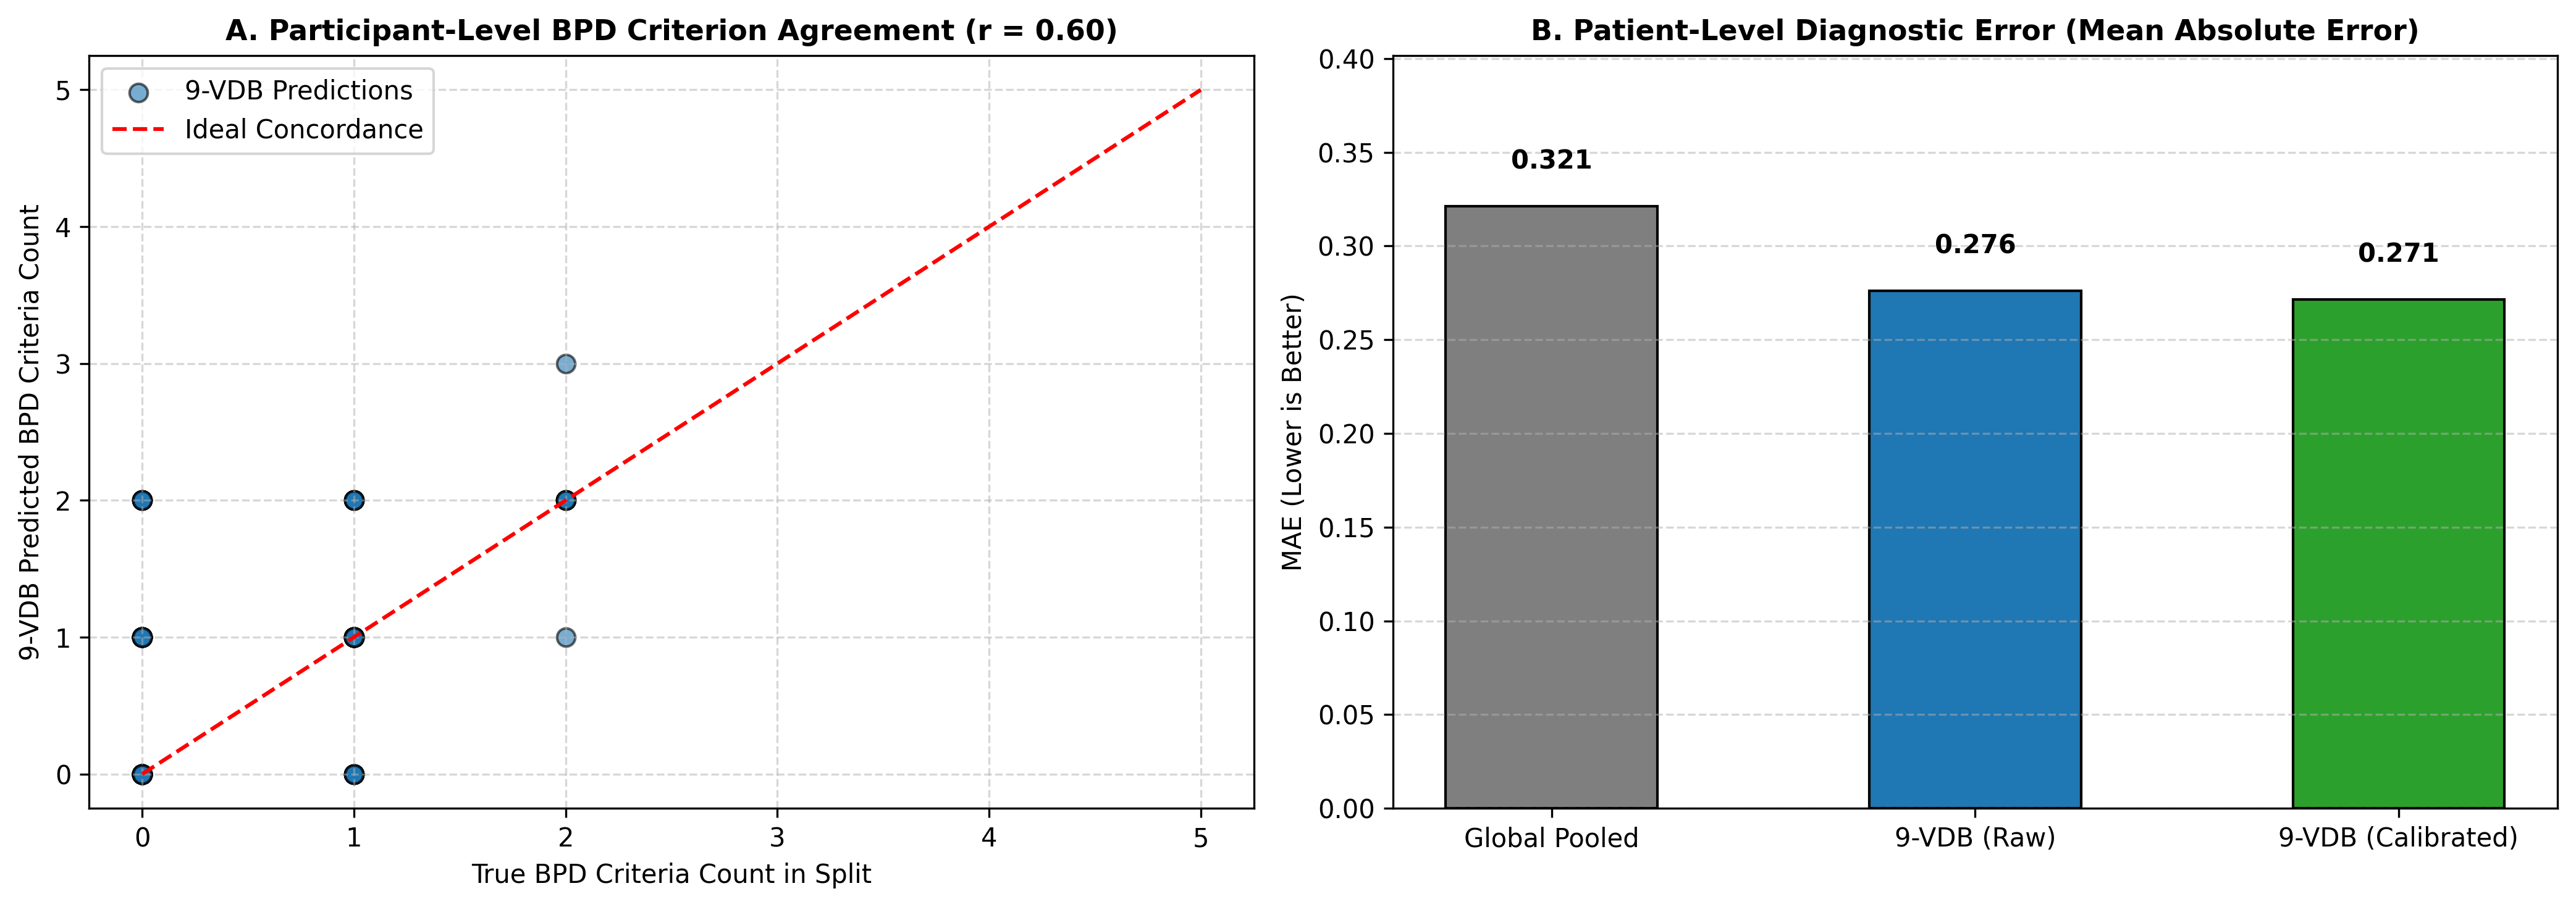
\includegraphics[width=0.85\textwidth]{figures/vbri/patient_level_diagnostic_agreement.png}
\caption{Patient-level diagnostic agreement: predicted versus true BPD criterion counts across
221 participants.}
\label{fig:patient_level}
\end{figure}

\subsection{Binary Clinical Screening}

Under the MSI-BPD binary screening protocol (BPD versus non-BPD), the 9-VDB Hybrid
configuration achieves the clinical metrics shown in Table~\ref{tab:screening}. The 95.96\%
negative predictive value means that when the system clears a patient as non-BPD, it is correct
96\% of the time. The diagnostic odds ratio of 26.52 indicates that a positive result is 26.5
times more likely to come from a true BPD case than from a non-BPD individual.

\begin{table}[H]
\centering
\caption{Binary clinical screening under the MSI-BPD protocol ($N = 333$).}
\label{tab:screening}
\small
\begin{tabular}{@{}lc@{}}
\toprule
\textbf{Metric} & \textbf{Value} \\
\midrule
Diagnostic Accuracy               & 81.68\% \\
Clinical Sensitivity (BPD Recall) & \textbf{86.57\%} \\
Clinical Specificity              & 80.45\% \\
Positive Predictive Value         & 52.73\% \\
Negative Predictive Value         & \textbf{95.96\%} \\
Diagnostic Odds Ratio             & \textbf{26.52} \\
\bottomrule
\end{tabular}
\end{table}

% =============================================================================
% 7. DISCUSSION
% =============================================================================
\section{Discussion}\label{sec:discussion}

The central finding of this work is that embedding-based semantic search can match the BPD
diagnostic sensitivity of the best fine-tuned transformer model, but does so with zero training
time, roughly 1,000 times lower inference latency, and full prediction explainability through
retrieved neighbours. This is a meaningful result for clinical deployment: in psychiatric triage,
sensitivity is the primary metric because a missed BPD case means a patient who needed
evaluation did not receive it. On this metric, \vbri{} is competitive with the strongest
available fine-tuned models at a fraction of the computational cost.

The gap in overall accuracy between \vbri{} and ModernBERT (72.97\% vs.\ 85.89\%) is real but
largely explainable. Fine-tuned models learn a decision boundary that is calibrated to the
three-way distinction between Normal, BPD, and Inconclusive, giving them an advantage on the
ambiguous Inconclusive class. \vbri{} relies on the structure of the training data, and the
semantic space does not always clearly separate sub-threshold emotional distress from clinically
diagnosable pathology. For tasks where this three-way accuracy is critical, fine-tuned models
remain the better choice. For settings where BPD sensitivity is the primary goal and
computational resources are limited, \vbri{} provides an effective and explainable alternative.

The error analysis identified the main remaining challenges. Negation blindness is the most
significant: embedding models encode ``I never tried to hurt myself'' and ``I tried to hurt
myself'' as semantically similar because the embedding space captures co-occurring vocabulary but
does not reliably encode logical negation. This caused 41 of the 91 total errors to be
Normal-to-BPD false positives. Identity disturbance (Q3) and proportionate anger responses (Q8)
were also difficult, since normal identity questioning and ordinary frustration share surface
vocabulary with their pathological counterparts. Addressing negation in clinical embedding models
is an important open problem for future work. The architecture is designed to be generalised, and
any clinical interview protocol that produces criterion-labelled responses can be adapted to the
\vbri{} framework.

% =============================================================================
% 8. CONCLUSION
% =============================================================================
\section{Conclusion}\label{sec:conclusion}

This paper introduced Vector-Based Retrieval Inference (\vbri{}), a training-free architecture
for clinical text classification that constructs nine criterion-isolated, class-balanced vector
databases from the \bpdqac{} dataset and classifies patient responses via similarity-weighted
nearest-neighbour voting. Through an iterative experimental process, we identified cross-question
semantic contamination and per-criterion class imbalance as the two key failure modes of naive
global retrieval, and resolved both through criterion isolation and 1:1:1 balanced curation. The
resulting system, enhanced with confidence calibration and a C-SSRS safety guard, achieves
86.57\% BPD sensitivity, identically matching the best fine-tuned transformer model, while
requiring no training time, running at 0.08\,ms per query (roughly 1,000 times faster), and
providing full prediction explainability through retrieved clinical precedents. These results
suggest that structured semantic search is a viable, transparent, and computationally efficient
approach for BPD screening and, more broadly, for clinical NLP tasks where diagnostic sensitivity
is the primary criterion and computational resources are constrained.

\section*{Data Availability}

The \bpdqac{} dataset is available at \textless{}repository link\textgreater{} as a CSV file
containing unique identifiers, question texts, participant responses, expert-annotated labels,
and binary indicators for Criteria B through F. The nine-VDB publication package including all
model artefacts, audit files, per-criterion reports, and reproducibility scripts is provided as
supplementary material.

\printbibliography

\end{document}
